\documentclass[12pt]{article}

\usepackage{hkueee}
\usepackage[T1]{fontenc}
\usepackage{hyperref}
\usepackage{url}
\usepackage{booktabs}
\usepackage{amsfonts}
\usepackage{nicefrac}
\usepackage{microtype}
\usepackage{amsmath}
\usepackage{cleveref}
\usepackage{lipsum}
\usepackage{graphicx}
\usepackage{natbib}
\usepackage{doi}
\usepackage{algpseudocode}
\usepackage{algorithm}
\usepackage{algpseudocode}
\usepackage{listings}
\usepackage{xcolor}
\usepackage{graphicx}
\usepackage{fontspec}
\setmainfont{Times New Roman}
\newfontfamily\chinesefont{Noto Serif TC}
\usepackage{setspace}
\usepackage{nomencl}
\makenomenclature

\hypersetup{
  pdftitle={\@title},
  pdfauthor={\@author},
}

% metadata for the  project
\courseproject{The project course title here}
\title{Your title here}
\author{Your name here}
\uid{Your UID here}
\supervisor{Your supervisor's name here}
\secondexaminer{Your second examiner's name here}


\begin{document}

\maketitle
\frontmatter
\begin{abstract}
  \lipsum[1]
\end{abstract}

\begin{acknowledgment}
  \lipsum[1]
\end{acknowledgment}

\makefrontmatter
\addcontentsline{toc}{section}{Nomenclature}
\printnomenclature

% list your abbreviation here
\nomenclature{AI}{Artificial Intelligence}
\nomenclature{ML}{Machine Learning}


\mainmatter
\newpage
\section{Introduction}

\subsection{Background}
\lipsum[1-3]

\subsection{Project Goal}
Goals of the project are:
\begin{itemize}
  \item Your first project goal.
  \item Your second project goal.
  \item Your third project goal.
\end{itemize}

\subsection{Report Organization}
\lipsum[1]

\section{Section}
\lipsum[1] \cite{kour2014real}

\subsection{Subsection 1}
\lipsum[1]

\subsubsection*{Subsubsection 1}
\lipsum[1]
\begin{table}[ht]
  \centering % Centers the table
  \begin{tabular}{l|c|r} % Specifies alignment for each column (left, center, right)
    \hline
    \textbf{Item} & \textbf{Quantity} & \textbf{Price} \\ \hline % Table header
    Apples        & 4                 & \$1.00         \\
    Oranges       & 5                 & \$1.50         \\
    Bananas       & 3                 & \$2.00         \\ \hline
  \end{tabular}
  \caption{Demo Table of Fruits} % Table caption
  \label{tab:fruits} % Label for referencing the table
\end{table}


\subsubsection*{Subsubsection 2}
\lipsum[1]
\begin{figure}[htbp]
  \centering
  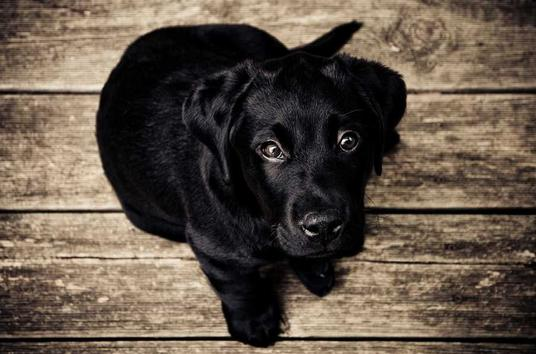
\includegraphics[width=0.9\textwidth]{assets/dog.jpg}
  \caption{Describe your figure with a caption.}
  \label{fig:dog} % use a unique label for each figure
\end{figure}


\subsection{Subsection 2}

\section{Conclusion}
\lipsum[1]

\subsection{Limitations}
\lipsum[1-2]


\backmatter
\makereferences
\appendix
\section{Appendix A}
\lipsum[1]


\end{document}
